\documentclass[specification,annotation]{itmo-student-thesis}

%% Опции пакета:
%% - specification - если есть, генерируется задание, иначе не генерируется
%% - annotation - если есть, генерируется аннотация, иначе не генерируется
%% - times - делает все шрифтом Times New Roman, требует пакета pscyr.

%% Делает запятую в формулах более интеллектуальной, например: 
%% $1,5x$ будет читаться как полтора икса, а не один запятая пять иксов. 
%% Однако если написать $1, 5x$, то все будет как прежде.
\usepackage{icomma}


%% Указываем файл с библиографией.
\addbibresource{bachelor-thesis.bib}

\begin{document}

\studygroup{M3439}
\title{Поиск абелевых строк наибольшей длины}
\author{Збань Илья Константинович}{Збань И.К.}
\supervisor{Аксёнов Виталий Евгеньевич}{Аксёнов В.Е.}{магистр}{аспирант Университета ИТМО/INRIA PARIS}
\publishyear{2017}
%% Дата выдачи задания. Можно не указывать, тогда надо будет заполнить от руки.
\startdate{01}{сентября}{2016}
%% Срок сдачи студентом работы. Можно не указывать, тогда надо будет заполнить от руки.
\finishdate{31}{мая}{2017}
%% Дата защиты. Можно не указывать, тогда надо будет заполнить от руки.
\defencedate{20}{июня}{2015}

%\addconsultant{Белашенков Н.Р.}{канд. физ.-мат. наук, без звания}
%\addconsultant{Беззубик В.В.}{без степени, без звания}

\secretary{Павлова О.Н.}

%% Задание
%%% Техническое задание и исходные данные к работе
\technicalspec{Улучшить существующие алгоритмы поиска наибольшей Абелевой подстроки, проанализировать существующие решения}

%%% Содержание выпускной квалификационной работы (перечень подлежащих разработке вопросов)
\plannedcontents{Тестирование на практике оптимального на данный момент алгоритма поиска абелевых подквадратов и работа над алгоритмами поиска НОАП}

%%% Исходные материалы и пособия 
\plannedsources{Опубликованные за последние годы публикации об абелевых строках}

%%% Календарный план
\addstage{Изучение предметной области}{09.2016}
\addstage{Проверка известных теоретических методов на компьютере}{11.2016}
\addstage{Постановка конкретных задач}{12.2016}
\addstage{Разработка алгоритмов для решения поставленных задач}{03.2017}
\addstage{Написать пояснительную записку}{05.2017}

%%% Цель исследования
\researchaim{Получить новый алгоритм поиска НОАП, улучшающий существующие результаты}

%%% Задачи, решаемые в ВКР
\researchtargets{Тестирование существующих алгоритмов, теоретическая и практическая оценка матожидания НОАП случайных строк, решение задачи о поиске НОАП в общем случае}

%%% Использование современных пакетов компьютерных программ и технологий
\advancedtechnologyusage{c++, python, gnuplot, git, etc}

%%% Краткая характеристика полученных результатов 
\researchsummary{Главным итогом работы является новый алгоритм поиска НОАП, на данный момент являющийся оптимальным по затратам времени и памяти}

%%% Гранты, полученные при выполнении работы 
\researchfunding{Грантов при выполнении работы получено не было}

%%% Наличие публикаций и выступлений на конференциях по теме выпускной работы
\researchpublications{Публикаций и выступлений на конференциях по теме выпускной работы не было}

%% Эта команда генерирует титульный лист и аннотацию.
\maketitle{Бакалавр}

\tableofcontents
%% Макрос для введения. Совместим со старым стилевиком.
\startprefacepage
%\newpage
%\section{Введение}

В последнее время стало появляться множество работ на тему Абелевой эквивалентности строк. Первые статьи на эту тему (?я нашел?) опубликованы около пятнадцати лет, и с тех пор наука шагнула далеко вперед в этом направлении.

Задачи данного типа встречаются в широком классе областей. Так, \textit{jumbled indexing} находит применение в бионформатике, при решении задач \textit{mass spectrometry} и \textit{gene clusters}. Кроме того, Абелево совпадение слов~--- хороший критерий эвристического фильтра для \textit{exact matching} и поиска с ошибками.

В главе 1 будут рассмотрены основные определения, используемые в работе, и известные на сегодняшний день результаты.

В главе 2 будут предложены новые алгоритмы и оценки на задачи по данной теме.

В главе 3 будут приведены практические результаты предложенных алгоритмов.
% Это одна из самых сложных частей. Здесь надо будет написать про мотивацию, описать предыдушие работы и поставить задачу.

\chapter{Обзор}
\section{Используемые определения}

Введем набор определений, которые будут использоваться по ходу работы. 

\begin{definition}
Алфавит $\Sigma=\{c_1, c_2, \ldots, c_\sigma\}$~--- конечное множество символов. Количество символов алфавита $|\Sigma|=\sigma$.
\end{definition}

\begin{definition}
$|s|_{c_1}$~--- количество символов $c_1$ в строке $s$.
\end{definition}


\begin{definition}
$\mathcal{P}(s)=(|s|_{c_1}, |s|_{c_2}, \ldots, |s|_{c_\sigma})$~--- вектор Парея, вектор частот символов строки $s$.
\end{definition}

\begin{definition}
$a \equiv b$, если $\mathcal{P}(a) = \mathcal{P}(b)$~--- Абелева эквивалентность двух строк. Две строки Абелево эквивалентны, если существует перестановка, переводящая одну из строк в другую.
\end{definition}

\begin{definition}
Строка $s$ является Абелевым квадратом, если существуют две Абелево эквивалентные строки $a \equiv b$, что $s = ab$.
%$s$~--- Абелев квадрат, если $s=ab$, где $a \equiv b$.
\end{definition}

\begin{definition}
Абелев подквадрат строки $s$~--- подстрока строки $s$, являющаяся Абелевым квадратом.
\end{definition}

\begin{definition}
\texttt{w.h.p.}~--- \textit{with high probability}, решение, с большой вероятностью работающее за такое время.
\end{definition}
%TODO WARNING переписать?

\begin{definition}
Будем говорить, что алгоритм работает за $\langle \mathcal{O}(f(n)), \mathcal{O}(g(n)) \rangle$, если он работает, используя $\mathcal{O}(f(n))$ времени и  $\mathcal{O}(g(n))$ памяти.
\end{definition}

\begin{definition}
\textit{НОАП} (\textit{LCAF})~--- наибольшая общая Абелева подстрока (longest common Abelian factor).
\end{definition}

\begin{problem}
$3SUM^+$: дано три множества целых чисел $A, B, C$, нужно найти три числа $a \in A, b \in B, c \in C$ такие, что $a+b=c$.
\end{problem}

\begin{problem}
%Поиск НОАП: даны две строки $a, b \in \Sigma^n$. Нужно найти наидлиннейшую строку $x$ такую, что $xs_a \equiv a, xs_b \equiv b$ для некоторых $s_a, s_b$.
Поиск НОАП: даны две строки $a, b$ над алфавитом $\Sigma$, нужно найти такие подстроки $x$ строки $a$ и подстроку $y$ строки $b$, что $x \equiv y$, а длина подстрок максимальна.
\end{problem}

\begin{problem}
Число Абелевых подквадратов: дана строка $s=s_0s_1 \ldots s_{n-1}$ над алфавитом мощности 2, $\Sigma = \{c_0, c_1\}$. Нужно найти количество различных ее подстрок $s_{i \cdots j}$, являющихся Абелевыми квадратами.
\end{problem}

\begin{problem}
\textit{Jumbled indexing}~--- задача проверки, содержит ли данный текст $T$ подстроку, Абелево эквивалентную шаблону $S$.
\end{problem}



%\begin{problem}

%\end{problem}

%Еще что-нибудь наверн
\section{Предыдущие результаты}
\subsection{Наибольшая общая Абелева подстрока}
Постановка задачи о поиске наибольшей общей Абелевой подстроке схожа с задачей поиска наидлиннейшей общей подстроки~--- очень важной задачи, исследовавшейся в 70-е года прошлого века. В частности, суффиксное дерево и линейный алгоритм его построения были разработаны в процессе работы над несколькими задачами, одной из которых являлся линейный поиск наидлиннейшей общей подстроки.

Задача поиска наибольшей общей Абелевой подстроки (\textit{LCAS}) была сформулирована в 2013 году на семинаре StringMasters. Там она была поставлена как открытая задача. 

После этого в 2015 году A.Attabi et al \cite{1} предложили два алгоритма решения этой задачи. 

Первый алгоритм решает задачу поиска НОАП за $\langle \mathcal{O}(n^2 \sigma), \mathcal{O}(n \sigma) \rangle$. В этом алгоритме авторы предлагают для каждой длины посчитать для обеих строк векторы Парея всех подстрок такой длины за $\langle \mathcal{O}(n \sigma), \mathcal{O}(n \sigma) \rangle$, отсортировать их сортировкой подсчетом, и после этого двумя указателями проверить, есть ли две Абелево эквивалентные подстроки.

Второй алгоритм решает задачу поиска НОАП для строк на бинарном алфавите. Он использует два факта: что для фиксированной длины подстроки достаточно сравнивать лишь количество одного из символов $c_1$, и что если у строки есть подстрока длины $l$ содержащая $x$ символов $c_1$, и подстрока длины $l$ содержащая $y$ символов $c_1$, то найдется и подстрока содержащая $z$ символов $c_1$ для любого $x \le z \le y$. Используя два этих факта, в алгоритме для обеих строк считается максимальное и минимальное количество символов $c_1$, которые могут быть у подстроки длины $l$ для каждой длины. Если эти отрезки для длины $l$ у строк пересекаются, то $l$~--- кандидат на НОАП. На алгоритм подсчета этих отрезков за $\mathcal{O}(n^2 / \log n)$ авторы ссылаются как на уже известный. Один из вариантов это сделать~--- применить метод четырех русских, предподсчитав матрицу размера $\log n \over 2$ на $\log n \over 2$, в которой содержится изменение количества единиц и максимальное число единиц, полученное на префиксе, если отрезать такие первые $\log n \over 2$ символов и дописать такие последние $\log n \over 2$ символов. Прыжков получится $2 \cdot n / \log n$, что и дает искомую асимптотику в $n^2 / \log n$.

В 2016 году на конференции SPIRE S.Grabowski et al \cite{4} улучшили алгоритм из \cite{1} 2015 года, уменьшив требование памяти до $\mathcal{O}(n)$, и предложили алгоритм, решающий задачу для случая алфавитов большого размера, работающий за $\langle \mathcal{O}(n^2 \log^2 n \log^* n), \mathcal{O}(n \log^2 n) \rangle$ времени и памяти. 

Первый результат, улучшение памяти алгоритма A.Attabi et al основано на двух оптимизациях. Во-первых, во время сортировки не хранятся все векторы Парея, а на каждой из $\sigma$ итераций количество вхождений очередного символа вычисляется заново. Во-вторых, для того, чтобы все еще можно было сравнивать векторы Парея, явно хранятся векторы Парея для всех позиций, кратных $\sigma$, т.е. для подстрок $s_0 \ldots s_{l-1}$, $s_\sigma \ldots s_{\sigma + l - 1}$, и так далее. Для сравнения векторов Парея двух произвольных подстрок, нужно взять ближайший посчитанный вектор Парея и изменить в нем $\mathcal{O}(\sigma)$ элементов, таким образом сравнение все еще работает за $\mathcal{O}(\sigma)$.

Второй алгоритм использует технику для поддержания изменяющегося множества строк с операциями split, join и equality testing, опубликованной в \cite{9}.

%TODO расписать больше мотивации? всякая биоинформатика

Сравнительное времени работы этих алгоритмов можно увидеть в таблице 1.

\begin{table}[H]
\begin{center}
\begin{tabular}{|c|c|c|c|}
\hline
Год & Авторы & Время & Память \\
\hline
2015 & A. Alattabi et al & $\mathcal{O}(n^2 \sigma)$ & $\mathcal{O}(n \sigma)$ \\
\hline
2016 & S. Grabowski et al & $\mathcal{O}(n^2 \sigma)$ & $\mathcal{O}(n)$ \\
\hline
2016 & S. Grabowski et al & $\mathcal{O}(n^2 \log^2 n \log^* n)$ & $\mathcal{O}(n \log^2 n)$ \\
\hline
2017 & Данная работа & $\mathcal{O}(n^2 \log \sigma)$ & $\mathcal{O}(n)$ \\
\hline
\end{tabular}
\end{center}
\caption{Существующие детерминированные алгоритмы поиска НОАП}
\end{table}

Кроме того, нельзя не упомянуть о недетерминированных версиях решения этой задачи. Публикации, посвященные этому алгоритму не были найдены, так что назовем это фольклором.

Определим полиномиальный хеш последовательности $s=s_0s_1\ldots s_{|s|-1}$ как $h(s)=(\sum\limits_{i=0}^{|s|-1} s_i \cdot p^i) \mod{m}$ для выбранных параметров $p$ и $m$, где в качестве $m$ обычно берется простое число, а в качестве $p$ произвольное.

Фиксировав длину $l$, можно скользящим окном посчитать полиномиальный хеш последовательностей $\mathcal{P}(s_i\ldots s_{i+l-1})$ для всех подстрок длины $l$, начинающихся в $i \in [0, n-l]$, за $\mathcal{O}(n)$ времени.

Посчитав полиномиальные хеши векторов Парея всех подстрок обеих строк, можно проверить, есть ли совпадающие, используя хешмап. В случае совпадения хешей нужно произвести допольнительную проверку подстрок на Абелеву эквивалентность, поскольку совпадение полиномиальных хешей еще не гарантирует эквивалентность строк, хотя коллизия хешей векторов Парея очень маловероятна.

Оценить математическое ожидание времени работы такого алгоритма довольно сложно, но на практике он работает очень быстро, и есть все основания полагать, что математическое ожидание его времени работы $\mathcal{O}(n^2)$. На этот алгоритм была предложена задача на интернет-олимпиаду ИТМО в 2015 году \cite{6}.

\subsection{Наибольший Абелев подквадрат и количество Абелевых подквадратов строки}
Задачи о нахождении наидлиннейшего Абелево подквадрата и их количества были поставлены в 2016 году, с указанием на метод, опубликованный в том же году, позволяющий решать некоторые задачи, связанные с Абелевой эквивалетностью, за субквадратичное время \cite{5}.

\begin{definition}
%Строка $t$ является Абелевым периодом строки $s$, если $s$ представимо как конкатенация набора строк $t_1 t_2 \ldots t_k$, где для всех $i$ верно, что каждое $t_i$ Абелево эквивалентно $t$.
Подстрока $s_i s_{i+1} \ldots s_{i+k-1}$ является Абелевым периодом строки $s$, если существует такое $j$, что $s_i s_{i+1} \ldots s_{i+k-1} \equiv s_{i+k} s_{i+k+1} \cdots s_{i+2k-1} \equiv \ldots \equiv s_{i+(j-1)k} s_{i+(j-1)k+1} \ldots s_{i+jk-1}$, и как $s_0 \ldots s_{i-1}$, так и $s_{i+jk} \ldots s_{|s|-1}$ являются Абелевыми подстроками подстроки $s_i s_{i+1} \ldots s_{i+k-1}$.
\end{definition}

\begin{definition}
Строка $t$ является Абелевым бордером строки $s$, если префикс и суффикс длины $|t|$ строки $s$ Абелево эквивалентны $t$.
\end{definition}

\begin{definition}
Абелев бордер $t$ является Абелевым покрытием строки $s$, если Абелевы вхождения строки $t$ в $s$ покрывают полностью всю строку $s$.
\end{definition}

Авторы этой статьи предложили алгоритмы поиска длиннейшего/кратчайшего Абелевого подквадрата за $\mathcal{O}(n^2 / \log^2 n)$, поиска кратчайшего Абелевого периода за $\mathcal{O}(n^2 / \sqrt{\log n})$, поиска Абелевых бордеров строки за $\mathcal{O}(n^2 / \log^2 n)$ и поиска всех Абелевых покрытий строки за $\mathcal{O}(n^2 / \log n)$.

Так же недавно был опубликован новый алгоритм для решения задачи $3SUM^+$, используя методы аддитивной комбинаторики, решающий частный случай задачи значительно быстрее, чем за квадратичное время~--- за $\mathcal{O}(n^{1.86})$. С помощью этого алгоритма они показали, как отвечать на запросы \textit{histogram queries} за $\mathcal{O}(1)$ после предподсчета за $\mathcal{O}(n^{1.86})$.

\subsection{Обзор алгоритма решения 3SUM+}

Кратко рассмотрим алгоритм решения задачи $3SUM^+$, предложенный в \cite{2}. 

В упомянутой статье было предложено решение задачи $3SUM^+$ для монотонных линейно ограниченных множеств. Ограничимся случаем, когда множества $A, B, C$ состоят из точек в двумерном пространстве.

Сначала вводится функция $cell(a)$~--- все точки разбиваются по принадлежности к клеткам со стороной длины $l$, получая $(n/l)^2$ различных клеток, в которых могут находиться исходные точки. Кроме того, точки нормализуются так, что для любых точек $a \in A, b \in B$ верно, что $cell(a+b)=cell(a)+cell(b)$, это достигается путем решения четырех подзадач подзадач.

Ко множеству непустых клеток $A^* = \{cell(a)\ :\ a \in A\}$,  $B^* = \{cell(b)\ :\ b \in B\}$, $C^* = \{cell(c)\ :\ c \in C\}$ применяется \textit{BSG Corollary}, получая набор множеств $A_1^*, \ldots, A_k^*, B_1^*, \ldots, B_k^*$ и остаток $R^*$.

Для каждой клетки остатка $(a^*, b^*) \in R^*$ задача решается рекурсивно для множеств $\{a \in A\ :\ cell(a)=a^*\}$, $\{b \in B\ :\ cell(b)=b^*\}$ и $\{c \in C\ :\ cell(c)=a^*+b^*\}$.

Затем, для каждого $i=1, \ldots, k$ применяется алгоритм, работающий на основе быстрого преобразования Фурье, чтобы получить все $\{a \in A\ :\ cell(a) \in A_i^*\}+\{b \in B\ :\ cell(b) \in B_i^*\}$, которые содержатся в надмножестве $T_i=\{s \in \mathcal{Z}^d\ :\ cell(s) \in A_i^* + B_i^*\}$.

Основная идея алгоритма в том, что после кластеризации точек, используя \textit{BSG Corollary} можно довольно быстро выделить набор пар множеств с малой декартовой суммой, которые своей суммой плотно покрывают кластеризованное точек, оставляя небольшой остаток. Для каждой непокрытой пары из остатка задача решается рекурсивно, а для каждой пары множеств, из-за того, что их декартова сумма невелика, используя быстрое преобразование Фурье, она считается быстрее, чем за квадрат.

Предложенный алгоритм является довольно большим продвижением в изучении задачи $3SUM^+$, являясь первым строго субквадратичным ($\mathcal{O}(n^\alpha), \alpha < 2$) алгоритмом для задач, основанных на ограниченной монотонной (min,+) свертке.

В алгоритме есть пространство для дальнейшего исследования. Так, авторами поставлена задача для улучшения детерменированной версии алгоритма с целью избавления от перемножения матриц с предположением, что можно так же использовать преобразование Фурье. Помимо этого, поиск применений мощных методов аддитивной комбинаторики в задачах дискретной математики выглядит очень перспективной областью исследования.


\chapter{Теоретические исследования}
\section{Абелевы квадраты}
% Мы расскажем в этой части как искать число бла-бла-бла.
% Так же мы провели эксперименты - правда ли n^1.8, и имеет ли вообще смысл такой алгоритм на практике

\subsection{Обзор алгоритма решения 3SUM+}

Кратко рассмотрим алгоритм, предложенный в \cite{2}. 

В этой статье предложено решение задачи $3SUM^+$ для монотонных линейно ограниченных множеств. Оно основано на использовании \textit{BSG-теоремы} и быстрого преобразования фурье для выделения набора пар подмножеств с относительно небольшой декартовой суммой, достаточно плотно покрывающих полную декартову сумму $A+B$.

Предложенный алгоритм является довольно большим продвижением в изучении задачи $3SUM^+$, являясь первым строго субквадратичным алгоритмом для задач, основанных на ограниченной монотонной (min,+) свертке.

В алгоритме есть большое пространство для дальнейшего исследования. Так, авторами поставлена задача для улучшения детерменированной версии алгоритма с целью от избавления от перемножения матриц с предположением, что можно так же использовать преобразование фурье. Кроме того, поиск применений мощных методов аддитивной комбинаторики в задачах дискретной математики выглядит очень перспективной областью исследования.

\subsection{Поиск числа Абелевых подквадратов}

\subsubsection{Сведение к 3SUM+}
Задачу о поиске числа Абелевых подквадратов бинарной можно свести к задаче 3SUM+.

Пусть строка . Рассмотрим следующие множества:

\begin{equation}
A = \{ (cnt_a(i), cnt_b(i)) | 0 \le i \le n \},
\end{equation}

\begin{equation}
B = \{ (cnt_a(i), cnt_b(i)) | 0 \le i \le n \},
\end{equation}

\begin{equation}
C = \{ (2cnt_a(i), 2cnt_b(i)) | 0 \le i \le n \},
\end{equation}


где $cnt_x(i)$~--- количество символов типа $c$ на префиксе строки $s$ длины $i$. Мотивация для этого сведения в том, что мы хотим, чтобы по обоим символам количество вхождений этого символа в первой половине строки было равно количеству вхождений во второй. Если рассматривать подстроку $[i; j)$, середина которой $k={i+j} \over 2$, то должно быть выполнено $cnt_a(k)-cnt_a(i)=cnt_a(j)-cnt_a(k)$ и $cnt_b(k)-cnt_b(i)=cnt_b(j)-cnt_b(k)$, или $cnt_x(i)+cnt_x(j)=2cnt_x(k)$. Поскольку $cnt_a(i)+cnt_b(i)=i$, становится понятно, что число абелевых подквадратов можно найти по формуле 

\begin{equation}
(\#3SUM^+(A, B, C) - (n+1)) / 2,
\end{equation}

где $n+1$ приходится вычитать, потому что нам неинтересны решения длины 0, а делить на два, потому что каждая подстрока будет посчитана дважды, с $i<j$ и $i>j$.

Поскольку лучшее известное решение задачи $3SUM^+$ для монотонных ограниченных $\mathcal{O}(n)$, работает за $\mathcal{O}(n^{1.86})$, а сведение работает за линию, получаем такое же решение задачи о количестве Абелевых подквадратов.

На самом деле, предполагая, что средний компьютер выполняет порядка $10^9$ операций в секунду, и предположив, что мы будем проверять решение на ограничениях порядка $n=10^5$, асимптотическое ускорение в $n^0.14$ переводя в числа ускоряет всего в ${10^5}^{0.14} \approx 5$ раз, что может оказаться незаметным, а вспоминая о большой константе алгоритма и нескольких логарифмах можно предположить о его практической неэффективности. Все же, представляет интерес для изучения работа алгоритма на специфичных тестах или в среднем случае, вдруг он работает достаточно быстро с какой-то стороны.
% Здесь рассказываешь в деталях как же ты ищешь

%\subsection{Реализация алгоритма}
% Тут можно описать все детали и проблемы, с которыми ты столкнулся в реализации.
% Далее, рассказать какие ты тесты генерировал И нарисовать красивый графичек.

\section{Наибольшая общая абелева подстрока}
% Описываешь задачу

\subsection{Общий алгоритм}

Отметим, что нас интересует детерменированный алгоритм решения задачи. Известно несколько недетерменированных решений, на практике работающих достаточно быстро, но они не являются темой исследования данной работы.

Будем подходить к лучшему решению по шагам от самого простого, на каждом шаге оптимизируя какую-то часть алгоритма, для лучшего понимания.

\subsubsection{$\langle \mathcal{O}(n^2 \log \sigma), \mathcal{O}(n \log \sigma) \rangle$ w.h.p}

Будем перебирать длину $l$ и проверять, есть ли общая абелева подстрока длины $l$.
План: построить $\mathcal{P}(t)$ для всех подстрок $t$ длины $l$ строк $a$ и $b$, потом понять, есть ли две строки с одинаковым $\mathcal{P}(t)$.

Будем строить векторы $P(t)$ для всех подстрок длины $l$ строк $a$ и $b$ по очереди, переходя от одной подстроки к следующей. Для этого нужно уметь удалять первый символ текущей строки и дописывать в конец новый символ. Расширим алфавит на один символ, добавив разделитель $\$$, нигде ранее не встречающийся, и будем идти скользящим окном длины $l$ по строке $a\$b$.

Хранить векторы $P(t)$ будем в персистентном массиве, реализованном на персистентном дереве отрезков. Для того, чтобы перейти к следующей подстроке, нужно уменьшить значение в одной ячейке на 1, и увеличить значение в другой ячейке на 1.

Для того, чтобы научиться сравнивать на равенство две вершины дерева, соответствующие двум векторам $P(t)$, будем при построении считать некоторое число $h(v)$~--- класс эквивалентности вершины. Этот класс эквивалентности будет соответствовать набору значений на подотрезке, соответствующему этой вершине~--- две вершины в одном классе эквивалентности, если они соответствуют одному и тому же подотрезку символов, и количество вхождений каждого символа у них одинаково.

Будем поддерживать хешмап, в котором для пары чисел $\langle h_1, h_2 \rangle$ хранится класс эквивалетности пары этих чисел, если она уже встречалась. Чтобы посчитать хеш для листа, проверим класс эквивалентности у пары $\langle -pos, val \rangle$, где $pos$~--- номер символа, соответствующего этому листу, а $val$~--- значение, записанное в этой вершине. Такая пара, с отрицательным $-pos$, выбирается для того, чтобы избежать коллизии со внутренними вершинами, характеристиками которых являются пары неотрицательных чисел~--- пара уже посчитанных классов эквивалентности сыновей $\langle h(v_l), h(v_r) \rangle$. Когда нам нужно узнать хеш пары $\langle h_1, h_2 \rangle$, смотрим в хешмап: если там есть элемент с таким ключом, то соответствующий класс эквивалентности уже посчитан, иначе кладем туда новый элемент с таким ключом и значением, равным размеру хешмапа. Значения всех хешей таким образом будут принимать значения от $0$ до $MapSize - 1$.

Таким образом, после подсчета класса эквивалентности каждой вершины, для всех подстрок длины $l$ первой и второй строки можно выписать их классы эквивалентности, и нужно проверить, есть ли в двух массивах одинаковое число. Поскольку все значения имеют порядок $\mathcal{O}(n \log \sigma)$, это можно сделать используя сортировку подсчетом.

Время работы~--- $n$ итераций по $l$, и $\mathcal{O}(n \log \sigma)$ операций для каждой длины: каждая вершина дерева отрезков создается за $\mathcal{O}(1)$ w.h.p. используя хешмап. Расходуемая память $\mathcal{O}(n \log \sigma)$ на хранение дерева отрезков и хешмапа.


\subsubsection{$\langle \mathcal{O}(n^2 \log \sigma), \mathcal{O}(n^2) \rangle$ deterministic}

Посмотрим внимательнее на персистентное дерево отрезков из предыдущего решения. Это ациклический ориентированный граф, в котором каждая вершина имеет свой уровень (глубину) от $1$ до $\log \sigma$, при чем на каждой глубине по $\mathcal{O}(n)$ вершин.

Будем считать классы эквивалентности всех вершин, поднимаясь по уровням от листьев к корням, используя один хешмап размера $\mathcal{O}(n^2)$, который умеем очищать за $\mathcal{O}(1)$. Под хешмапом здесь и далее я подразумеваю просто массив на $\mathcal{O}(n^2)$ элементов с пометкой последнего изменения для возможности обнуления за $\mathcal{O}(1)$.

В этом решении класс эквивалентности будет будет иметь не сквозную нумерацию среди всех вершин дерева, как в предыдущем решении, а иметь отдельную нумерацию для каждого уровня вершин дерева.

База: посчитать классы эквивалентности листьев. Класс эквивалентности листа, как и в прошлом пункте, $h(\langle -pos, val \rangle)$, где и $pos$, и $val$ принимают значения порядка $\mathcal{O}(n)$. Поэтому можно пройти по всем листам в дереве, и посчитать классы, обращаясь к хешмапу напрямую и спрашивая, был ли уже такой же лист, и какой у него класс эквивалентности. Для того, чтобы обойти все листы за их количество, при построении дерева можно в каждый лист складывать ссылку на новый лист, который появляется в следующей версии дерева отрезков.

Переход: посчитан класс эквивалентности всех вершин более глубокого уровня. Обратим внимание, что поскольку на каждой глубине $\mathcal{O}(n)$ вершин, классы этих вершин так же будут принимать значения $\mathcal{O}(n)$. Поэтому мы можем очистить хешмап и точно так же, как и для листьев, считать значение класса, к которому относится вершина, проверяя, была ли уже такая пара $\langle h(v_l), h(v_r) \rangle$.

Таким образом, мы построили дерево и посчитали хеши всех вершин за $\langle n^2 \log \sigma, n^2 \rangle$ полностью детерменированно.


\subsubsection{$\langle \mathcal{O}(n^2 \log \sigma), \mathcal{O}(n) \rangle$ deterministic}

Начнем с того, что на хранение дерева отрезков у нас сейчас уходит $n \log \sigma$ памяти, это много. Чтобы уменьшить потребление памяти, можно использовать технику \textbf{limited node copying}. Краткое введение, которое будет необходимо для дальнейшего понимания алгоритма: %TODO где прочитать про эту технику?

Вместо того, чтобы после пересоздания очередного листа пересоздавать весь путь до корня, будем хранить в каждой вершине дополнительный указатель, изначально нулевой. При изменении значения в листе будем подниматься по предкам, пока у предка дополнительный указатель уже занят, и создавать в этом случае новую вершину. Когда мы стоим в вершине и знаем, что один из ее сыновей был изменен, а дополнительный указатель еще не занят, просто установим этот дополнительный указатель на новую версию этого сына и подпишем текущим глобальным временем. После такого изменения все еще несложно обратиться к какой-то версии дерева отрезков: нужно просто при переходе к сыновьям при выборе, куда спускаться, посмотреть, не нужно ли идти по дополнительному указателю.

Можно доказать, что таким образом построенное дерево занимает $\mathcal{O}(n)$ памяти, используя амортизационный анализ, но не будем об этом. 

Подсчет классов эквивалентности для листьев и внутренних вершин в этом решении отличается.

База: подсчет классов для листьев. Будем считать классы для листьев группами, для каждой позиции все листья, соответствующие этой позиции в массиве, вместе. Будем поддерживать счетчик $ch$~--- первый еще не использованный номер класса эквивалентности. Фиксировав, какую позицию мы сейчас обрабатываем, просто обойдем все листья с этой позицией (для этого можно хранить в каждом листе ссылку на предыдущий лист этой позиции), и листу со значением $val$ присвоим хеш $ch+val$. после чего увеличим $ch$ на $maxValue_{pos}+1$, где $maxValue_{pos}$~--- наибольшее значение, которое было в ячейке $pos$ в одной из версий дерева отрезков. Мы знаем $maxValue_{pos}$ для каждой позиции, и можно заметить, что количество классов эквивалентности на этом уровне $\mathcal{O}(n)$, поскольку $\sum \limits_{pos=0}^{\sigma} maxValue_{pos} = \mathcal{O}(n)$.

Переход: посчитали классы для всех (даже больше, чем для всех вершин, об этом далее) вершин на предыдущем уровне. Кроме класса вершины мы записываем не только эту вершину, а еще и все ее копии во все времена, которые мы не создавали явно в дереве отрезков (при переходе на послеследующий уровень их можно безопасно удалить, чтобы сохранить линейную память). Чтобы получить для вершины список всех времен, когда она должна была бы существовать без сжатия, нужно просто взять список всех времен всех трех ее сыновей и смерджить, это делается за линейное время, поскольку они уже отсортированы. 

Следующее, что нужно сделать~--- сгруппировать все вершины с одинаковым $h(v_l)$ в одну группу, и обработать их вместе, чтобы назначить им соответствующие классы эквивалентности. Пусть у очередной вершины (для каждого варианта глобального времени, которое в ней интересно) классы сыновей $h(v_l)$ и $h(v_r)$. Запишем в вектор с номером $h(v_l)$ напоминание: нужно посчитать $h(\langle h_1, h_2 \rangle)$ и записать его в текущую вершину $v$. После того, как сделали это для всех вершин текущего уровня, можно перебирать $h(v_l)$, очищать хешмап размера $\mathcal{O}(n)$, и перебирать соответствующее ему $h(v_r)$, назначая вершинам текущего уровня соответствующие классы. Как обычно, если $h(v_r)$ есть в хешмапе, достаем оттуда посчитанный класс, иначе сопоставляем ему новый. 

После того, как классы эквивалентности всех вершин посчитаны, можно освобождать память с предыдущего уровня и переходить к следующему. В конце получим посчитанные классы для всех корней.

Используемое время так и осталось $\mathcal{O}(n^2 \log \sigma)$, а вот требуемая память стала всего $\mathcal{O}(n)$.

Остается открытым вопрос существования более быстрых детерменированных алгоритмов, работающих за $o(n^2 \log \sigma)$, в частности, $\mathcal{O}(n^2)$. К существованию такого алгоритма есть такие предпосылки, как недетерменированные алгоритмы, работающие за $\langle \mathcal{O}(n^2), \mathcal{O}(n) \rangle$.

\subsection{Случай бинарных строк}
% Здесь описываешь алгоритм для бинарных строк
Отдельный интерес представляет случай $\sigma=2$. Есть известный алгоритм, описанный, например, в [1], работающий за время $O(n^2/\log n)$.

В этой же статье рассмотрена задача матожидания длины НОАП двух случайных строк длины $n$ и сделано предположение 5.1 о том, что $LCAF_{avg} \ge n - O(\log n)$. Это преположение выглядит слишком смелым, рассмотрим эту задачу подробнее.


\begin{theorem} %TODO сбилась нумерация теорем :(
Для любой функции $f(n)=o(n)$ верно что для двух случайных бинарных строк длины $n$: $LCAF_{avg} < n - f(n)$.
\end{theorem}
\begin{proof}
%От противного. Предположим, что есть функция $f(n)$ и некоторая константа $\alpha<1$ что $LCAF_{avg} >= n - f(n)$, и $f(n) = o(n^\alpha)$.

Лемма: для любой функции $f(n)=o(n)$ с вероятностью $P>0$ верно $LCAF_{avg} < n - f(n)$.

Обратим внимание, что центральная подстрока длины $n-2f(n)$, полученная отрезанием суффикса и префикса длины $f(n)$, является подстрокой любой строки длины $n-f(n)$ этой же строки.

Рассмотрим задачу как задачу случайного блуждания: пусть $x_i = A_i - B_i$, где $A, B$~--- наши случайные строки. От стандартной задачи случайного блуждания она отличается тем, что кроме переходов $|x_{i+1}-x_i|=1$ разрешены переходы $x_{i+1}=x_i$. Абелево равенство двух подстрок $A$ и $B$ эквивалентно тому, что подпуть блуждания $x$ возвращается в свое начало, $x_r=x_l$.

Наше случайное блуждание имеет следующие вероятности:

\begin{tabular}{|c|c|}
\hline
$\Delta x$ & $p(\Delta x)$ \\
\hline
-1 & 0.25 \\
\hline
0 & 0.5 \\
\hline
1 & 0.25 \\
\hline
\end{tabular}

$P(n, k)$~--- вероятность после $n$ испытаний получить сумму $k$. Можно заметить, что $P(n, k)=C(2n, n+k)\cdot 2^{-2n}$. И действительно, если посмотреть на геометрический смысл этого распределения, то $P(n,k)$~--- вероятность за $2n$ равновероятных шагов вправо или вверх дойти до диагонали $x+y=2n$ и остановиться на диагонали $y-x=k$, что сходится с формулой $P(n,k)=P(n-1,k-1)+2P(n-1,k)+2P(n-1,k+1)$.

При больших $n$ будем приближать наше биномиальное распределение нормальным, $P(n, k)=\sqrt {n} N(0,1)$ %TODO (WARNING, CHECK CONSTANT)

Вспомним о правиле трех сигм:

\begin{figure}[h]
\center{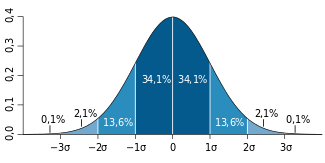
\includegraphics[scale=1]{pics/3sigm.png}}
\caption{правило трех сигм \cite{3}}
\end{figure}

Поскольку у нормального распределения $\sqrt {2n} N(0,1)$ среднеквадратичное отклонение $\sigma = \sqrt{n}$, по правилу трех сигм можно сказать, что у центрального пути длины $n-2f(n)$ вероятность остановиться в промежутке $[-3\sqrt{n-2f(n)}; 3\sqrt{n-2f(n)}]$ около 0.9973, а поскольку $f(n)=o(n)$, вероятность того, что изменение координаты окажется вне промежутка $[-3\sqrt{n}; 3\sqrt{n}]$, хотя бы 0.0026. %TODO (WARNING, считаю, что f(n)=o(n) ---> \_очевидно\_, что можно выкинуть f(n) оттуда)

Для того, чтобы получить отрезок длины $n-f(n)$ с нулевой суммой, нужно взять какой-то суффикс префикса длины $f(n)$ и какой-то префикс суффикса длины $f(n)$. Покажем, что с достаточной вероятностью мы не сможем приблизиться к нулю за $f(n)$ шагов:

Скажем, что наше блуждание сейчас будет обычным случайным, с двумя переходами +1 и -1. Этот переход лишь делает оценку строже, т.к. можно продлить все испытания, в которых был переход по 0 до ровно $k$ ненулевых переходов и прийти к случайному блужданию, при чем максимум модуля отклонения на префиксе мог только увеличиться.

%Есть известный факт, что в случайном блуждании если мы находимся в 0, и заканчиваем, когда попадем в точку с координатой $a$ или $-b$ ($0 < a, b$), то матожидание шагов до этого события $ab$. Воспользуемся этим: матожидание количества шагов до момента, когда мы попадем первый раз в точку $-\sqrt n$ или $\sqrt n$, равно $(\sqrt n)^2=n$. Поскольку матожидание равно $n$, значит существует вероятность $C>0$, с которой весь наш путь из $n$ шагов будет в полосе $(-\sqrt n, \sqrt n)$. %TODO (WARNING, доказательство не оч из-за $C$, надо поаккуратнее)

Поскольку $2f(n)=o(n)$, докажем более сильное условие. За $n$ шагов с вероятностью $C>0$ случайное блуждание не попадет в область с координатой меньше $-\sqrt{n}$. 

Переформулируем эту задачу как задачу о разорении: игрок имеет $\sqrt{n}$ денег и играет $n$ раундов против бесконечно богатого казино, и нужно найти вероятность разорения игрока. В \cite{7} и в \cite{8} можно найти следующую формулу: вероятность проигрыша игрока со стартовым капиталом $a$ за $n$ раундов равна $y_{a,n}=1-{{2} \over {\sqrt{\pi}}} \int_0^t e^{-u^2} du + \Delta$, где $\Delta$~--- малый остаточный член, а $t={{a} \over {\sqrt{2(n+{{2}\over 3})}}}$.

В нашем случае, $a=\sqrt n$, $t \approx {1 \over \sqrt 2}$, и вероятность проигрыша в пределе равна $1 - {2 \over \sqrt \pi}1 \int_0^{1 \over \sqrt 2} e^{-u^2} du \approx 0.395$.

Таким образом, с вероятностью хотя бы 0.0026 центральный подпуть будет иметь отклонение от нуля хотя бы в $3\sqrt n$, и с вероятностью хотя бы $0.395^2$ и префикс, и суффикс, который мы допишем к этой строке, будут иметь отклонение не больше, чем на $\sqrt n$, то есть, с вероятностью $P \ge 0.026 \cdot 0.395^2$ у двух случайных строк наибольшая абелева подстрока будет меньше, чем $n-f(n)$.

Вернемся к доказательству теоремы. Будем доказывать ее от противного~--- пусть есть $f(n)=o(n)$ такое, что $LCAF_{avg} \ge n - f(n)$. 

Оценим $LCAF_{avg}$. По лемме, с вероятностью $P>0$ $LCAF$ будет не больше, чем $g(n)=\sqrt{nf(n)}$. Тогда

$LCAF_{avg} \le P (n-g(n)) + (1-P)n = n-Pg(n) < n - f(n)$, т.к. $f=o(g)$. Противоречие.

\end{proof}

Кроме того, докажем грубую оценку снизу:
\begin{theorem}
Для двух случайных бинарных строк длины $n$: $LCAF_{avg} \ge 0.05n$.
\end{theorem}
\begin{proof}
Снова приблизим наше случайное блуждание нормальным распределением и воспользуемся правилом трех сигм.

С вероятностью $2 \cdot 0.34$ за первые $n/2$ шагов мы остановимся в зоне $[-\sigma; \sigma]$. После этого, с вероятностью хотя бы $0.136+0.021+0.001 \ge 0.15$ мы за следующие $n/2$ шагов пройдем в другую сторону хотя бы $\sigma$ шагов, обязательно перейдя через точку старта. Таким образом, с вероятностью хотя бы $2 \cdot 0.34 \cdot 0.15$ НОАП будет хотя бы $n/2$, или $LCAF_{avg} \ge 0.05$. %TODO может стоит \sigma -> \sqrt

\end{proof}

Итого, получаем, что матожидание НОАП у двух случайных бинарных строк сверху и снизу ограничено линейными функциями, но более точная оценка ее поведения остается нерешенной задачей.

%\end{table}

\chapter{Практические результаты}
\section{Параметры компьютера, производящего вычисления}
Все вычисления были выполнены на ноутбуке Acer с процессором Intel(R) Core(TM) i7-4710HQ CPU @ 2.50GHz.

Реализации всех алгоритмов были написаны на языке C++, и были скомпилированы с флагами $-O2$.

\section{Наибольшая общая Абелева подстрока}
\subsection{Случай бинарного алфавита}

Первое, что мы сделаем~--- посмотрим, как себя ведет на практике матожидание наибольшей общей Абелевой подстроки двух случайных бинарных строк. 

Мы выполнили $10^4$ запусков поиска НОАП для различных значений $n$ до $10^4$. Такого количества запусков оказалось вполне достаточно, чтобы среднее значение НОАП стабилизировалось. Полученный результат можно увидеть на рисунке 2.

\begin{figure}[h]
\center{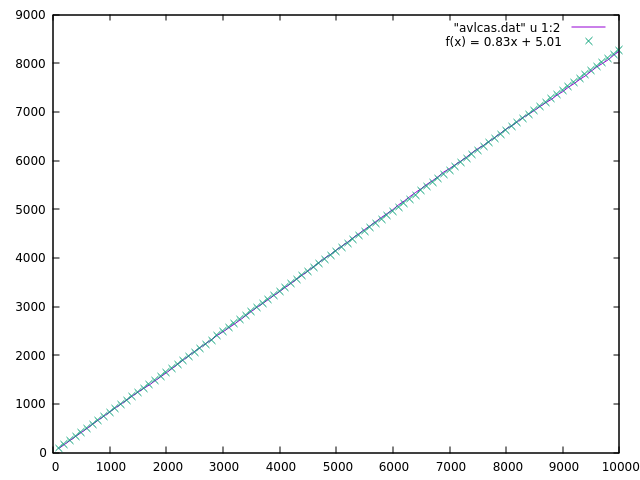
\includegraphics[scale=1]{pics/avlcas.png}}
\caption{зависимость матожидания НОАП от длин строк}
\end{figure}

Видно, что функция ведет себя очень точно как прямая $y=0.83x$, что подтверждает полученные теоретические линейные оценки как сверху, так и снизу.

%\subsection{Общий случай}
%Пусто? Ну я канеш могу закодить то что я придумал но не оч хочется(((

\subsection{Случай большого алфавита}

Будем сравнивать время работы предложенного в этой статье алгоритма за $\mathcal{O}(n^2 \log \sigma)$ с алгоритмом, предложенным A. Attabi et al \cite{1}. Главными достоинствами этого алгоритма является необычайная простота, котороая приводит к очень маленькой константе, скрытой во временной оценке, потому что в нем не используется никаких тяжелых алгоритмов. Алгоритм S. Grabowski et al \cite{4} за $\mathcal{O}
(n^2 \log \sigma)$ имеет такую же временную асимптотику, поэтому с ним сравнение не проводилось: есть все основания полагать, что он работает в несколько (как минимум, в два) раз медленнее из-за эвристик, приводящих к уменьшению потребления памяти.

Так же в процессе анализа я решил не сравнивать с алгоритмом S. Grabowski et al \cite{4} за $\mathcal{O}(n^2 \log^2 n \log^* n)$, потому что в процессе ознакомления с ним я решил, что у него слишком большая скрытая константа~--- алгоритм получен в результате деамортизации недетерменированного, используя для этого довольно тяжелые операции и структуры данных.

В свою очередь, алгоритм, предложенный в этой статье, достаточно тяжелый как в плане написания кода, так и имеет сложно оцениваемую скрытую константы времени работы из-за необходимости очень аккуратно работать с памятью. Представляет большой интерес узнать, является ли данный алгоритм лишь теоретическим улучшением существующих, или он дает ощутимое ускорение на практике.

Сравнение времени работы предложенного алгоритма в зависимости от $n$ на тесте, сгенерированном из двух строк длины $n$, состоящих из случайных символов из алфавита мощности $n$, представлено на рисунке 3.

\begin{figure}[h]
\center{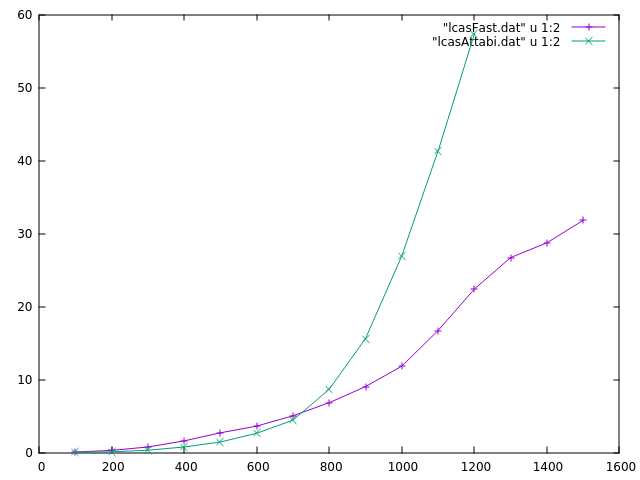
\includegraphics[scale=1]{pics/common_lcas_n.png}}
\caption{Зависимость времени работы алгоритмов от $n$ на случайной строке над большим алфавитом}
\end{figure}

Таким образом, можно с уверенностью сказать, что начиная с не очень большого $n$ предложенный алгоритм начинает сильно выигрывать у стандартной реализации известного алгоритма, и этот выигрыш будет только увеличиваться из-за более хорошей асимптотики.

К сожалению, несмотря на строго более хорошую асимптотику, для маленьких тестовых данных предложенный алгоритм работает несколько медленнее, чем стандартное решение. Это можно объяснить наличием скрытой в асимптотике алгоритма константой, но она достаточно мала, чтобы все равно обеспечить выигрыш на реальных данных.

\section{Количество Абелевых подквадратов}

Далее мы реализовали алгоритм нахождения числа Абелевых подквадратов с помощью сведения к алгоритму решения монотонного ограниченного случая $SUM^+$. Он был протестирован на строках из одинаковых символов, и на наборе пар случайных бинарных строк. Как оказалось, константа алгоритма довольно велика, и на практике он показал себя достаточно плохо, в несколько раз проигрывая наивному решению за $\mathcal{O}(n^2)$.

\begin{figure}[h]
\center{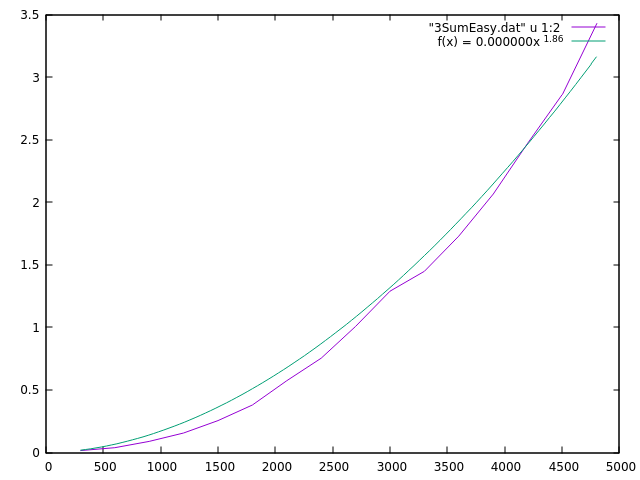
\includegraphics[scale=1]{pics/4.png}}
\caption{зависимость средней времени работы на унарной строке от ее длины}
\end{figure}

На рисунке 3 можно увидеть зависимость времени работы решения в секундах от $n$~--- длины строк, данных на вход, на тесте со строками из одинаковых символов. График действительно довольно похож на $n^{1.86}$, но из-за нескольких логарифмов в асимптотике растет несколько быстрее. 

\begin{figure}[h]
\center{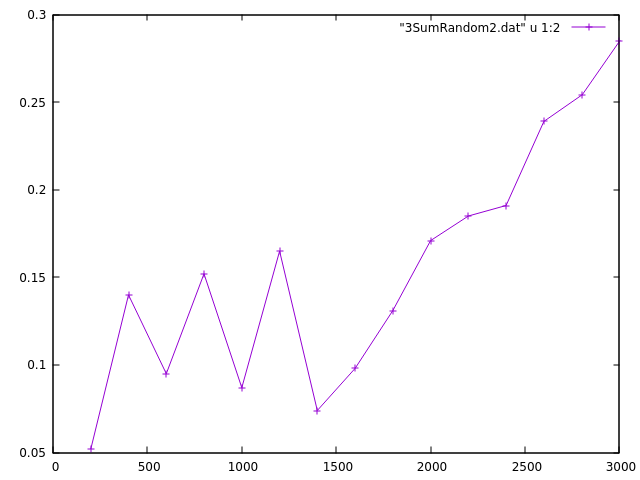
\includegraphics[scale=1]{pics/5.png}}
\caption{зависимость средней времени работы на случайной строке от ее длины}
\end{figure}

На рисунке 4 можно увидеть зависимость времени работы решения в секундах от $n$~--- длины строк, данных на вход, на тесте со случайными строками из двух различных символов.

Время работы алгоритма довольно сильно меняется как от запуска к запуску из-за разных тестов, так и от различных значений $n$, так как различные ветки программы выполняются с разными вероятностями и работают разное время~--- не приходится удивляться некоторому увеличению производительности при увеличении $n$.


%% Макрос для заключения. Совместим со старым стилевиком.
\startconclusionpage
%\section{Заключение}
% Здесь говоришь какой ты молодец и сколько всего сделал
Я протестировал асимптотически оптимальный алгоритм решения монотонного 3SUM и выяснил, что он медленный.

А еще придумал классные оценки для binary LCAS и улучшил оптимальный алгоритм для LCAS в общем случае.

%clearpage
%\begin{thebibliography}{99}
\addcontentsline{toc}{subsection}{Литература}

\bibitem{LCAF15}
{\it Ali Alatabbi, Costas S. Iliopoulos, Alsessio Langiu, M. Sohel Rahman,}
Algorithms for Longest Common Abelian Factors /\!/
International Journal of Foundations of Computer Science. – 2016. – Т. 27. – №. 05. - С.~529-543

\end{thebibliography}



%\cite{1}

%% После этой команды chapter будет генерировать приложения, нумерованные русскими буквами.
\printmainbibliography



\end{document}
